%%
%% This is file `./samples/longsample.tex',
%% generated with the docstrip utility.
%%
%% The original source files were:
%%
%% apa7.dtx  (with options: `longsample')
%% ----------------------------------------------------------------------
%% 
%% apa7 - A LaTeX class for formatting documents in compliance with the
%% American Psychological Association's Publication Manual, 7th edition
%% 
%% Copyright (C) 2021 by Daniel A. Weiss <daniel.weiss.led at gmail.com>
%% 
%% This work may be distributed and/or modified under the
%% conditions of the LaTeX Project Public License (LPPL), either
%% version 1.3c of this license or (at your option) any later
%% version.  The latest version of this license is in the file:
%% 
%% http://www.latex-project.org/lppl.txt
%% 
%% Users may freely modify these files without permission, as long as the
%% copyright line and this statement are maintained intact.
%% 
%% This work is not endorsed by, affiliated with, or probably even known
%% by, the American Psychological Association.
%% 
%% ----------------------------------------------------------------------
%% 
\documentclass[stu, floatsintext, helv]{apa7}

\usepackage{lipsum}

\usepackage{enumitem}

\usepackage[american]{babel}

\usepackage{tikz}
\usetikzlibrary{shapes.geometric, arrows, positioning, calc}
\usepackage{csquotes}
\usepackage{pdfpages}
\usepackage{float}
\usepackage{caption}
\usepackage{subcaption}
\usepackage{makecell}
\usepackage{placeins}
\usepackage[style=apa,backend=biber]{biblatex}
\addbibresource{bibliography.bib}


\renewcommand\theadalign{cc} % Zentriert den Text in der Kopfzeile
\renewcommand\theadfont{\bfseries} % Fettgedruckter Text für die Kopfzeile
\renewcommand\cellalign{l} % Setzt die Standardausrichtung von makecell auf linksbündig


\title{Gender Differences in the Impact of Gamification Elements on Performance and Anxiety}
\shorttitle{Gender Differences in the Impact of Gamification Elements}

%\authorsnames{Robin Gebert, Nadine Koch, Niklas Meißner, Jun.-Prof. Dr. rer. nat. Maria Wirzberger}
%\authorsaffiliations{University of Stuttgart}
\author{Robin Gebert}
\authorsaffiliations{University of Stuttgart}
\course{Informatik - B.A. (Lehramt)}
\professor{Jun.-Prof. Dr. rer. nat. Maria Wirzberger}
\advisor{Nadine Nicole Koch, M.Sc.\newline\noindent Niklas Meißner, M.Sc.}
\startdate{06. Mai 2024}
\enddate{06. September 2024}

\leftheader{Gebert}

\abstractGerman{Diese Bachelorarbeit untersucht die Auswirkungen verschiedener Gamification-Elemente auf Leistung und Angst in digitalen Lernumgebungen, mit einem besonderen Fokus auf Geschlechterunterschiede. Trotz der breiten Anwendung von Gamification in Bildungstechnologien ist das Verständnis darüber, wie individuelle Faktoren wie Geschlecht diese Effekte beeinflussen, begrenzt. Die Studie verwendet ein 2$\times$8 faktorielles Design, um die Interaktionen zwischen Gamification-Elementen und Geschlecht zu analysieren, wobei 117 Teilnehmer aus verschiedenen Studiengängen rekrutiert wurden. Die Ergebnisse zeigen, dass verschiedene Gamification-Elemente die Leistung und Angst unterschiedlich beeinflussen, jedoch waren diese Gruppenunterschiede überwiegend deskriptiv und nicht signifikant. Diese Erkenntnisse deuten darauf hin, dass die Anpassung von Gamification-Strategien an geschlechtsspezifische Reaktionen potenziell die Effektivität von digitalen Lernumgebungen verbessern könnte. Die Studie betont die Notwendigkeit weiterer Forschungen, um die Beziehung zwischen Gamification, Geschlecht und Lernausgängen tiefer zu verstehen.}
\keywordsGerman{Gamification, Geschlecht, Intelligente Tutorielle Systeme, Leistung, Angst}

\abstractEnglish{This bachelor thesis explores the effects of various gamification elements on performance and anxiety in digital learning environments, with a specific focus on gender differences. Despite the widespread application of gamification in educational technologies, understanding of how individual factors such as gender influence these effects remains limited. The study employed a 2$\times$8 factorial design to analyze interactions between gamification elements and gender, recruiting 117 participants from various degree programs. Findings indicate that different gamification elements variably affect performance and anxiety, however, these group differences were predominantly descriptive and not significant effects. These insights suggest that tailoring gamification strategies to gender-specific responses could potentially enhance the effectiveness of digital learning environments. The study underscores the need for further research to deepen understanding of the relationship between gamification, gender, and learning outcomes.}
\keywordsEnglish{Gamification, Gender, Intelligent tutoring systems, Performance, Anxiety}

%%
%%\authornote{
%%   \addORCIDlink{Daniel A. Weiss}{0000-0000-0000-0000}
%%
%%  Correspondence concerning this article should be addressed to Daniel A. Weiss, Department of Educational Psychology, Counseling and
%%  Special Education, A University Somewhere, 123 Main St., Oneonta, NY
%%  13820.  E-mail: daniel.weiss.led@gmail.com}
%%
\begin{document}
\maketitle


%
The often mandated transition to remote education during the COVID-19 pandemic highlighted the indispensable role of digital learning environments (DLEs) \parencite{garcia-moralesTransformationHigherEducation2021}.
The usage of digital learning resources saw a significant increase during this period; in 2019, 54\% of students utilized such resources, with the figure rising to 70\% in 2020.
In Germany, the percentage of scholars aged ten to fifteen engaging with digital learning materials doubled from 32\% to 64\% within the same timeframe \parencite{pressestelledesstatistischenbundesamtsDigitalesLernenNimmt2020}.

The integration of gamified elements into DLEs is a common practice, aimed at enhancing motivation and enjoyment \parencite{gonzalezGamificationIntelligentTutoring2014, jacksonMotivationPerformanceGamebased2013}.
However, despite the positive impacts, the introduction of some elements can also lead to negative outcomes, including demotivation \parencite{almeidaSystematicMappingNegative2021}.
The concept of gamification has attracted substantial interest within the educational sciences, becoming a prevalent topic \parencite{swachaStateResearchGamification2021}.
In the realm of computer science, the application of gamified elements is well-documented, demonstrating a important presence due to the inherent integration of technology in the field \parencite{dichevGamifyingEducationWhat2017}.

Although there is extensive research on the general application of gamification, the effects related to individual factors, such as gender, are less understood and warrant further investigation \parencite{dehghanzadehUsingGamificationSupport2024, oliveiraTailoredGamificationEducation2023}.


%% !TeX spellcheck = en_US
%The concept of grading can be seen as a form of gamification, as it adds feedback and a competitive element to the learning process.
%But in recent years especially with the advance of computers, gamification has become an increasingly popular topic in education science \parencite{swachaStateResearchGamification2021}.
%Especially in computer science the use of gamified elements is well researched \parencite{dichevGamifyingEducationWhat2017}, which could be related to the already great use of computers in the field.
%But as this field is still relatively new, many topics are still not well researched, especially how individual factors, such as gender, can influence the effects of gamification \parencite{dehghanzadehUsingGamificationSupport2024,oliveiraTailoredGamificationEducation2023}.
%This thesis aims to explore the effects of different gamified elements and their combinations on performance and anxiety in a digital learning environment, especially focusing on the influence of gender on these effects.
%Digital learning environments, or tutoring systems, were hugely affected by the shift of teaching to remote classes during the COVID-19 pandemic.
%In 2019, 54\% of students utilized digital learning materials, which increased to 70\% the following year. Meanwhile, only 32\% of German scholars aged ten to fifteen engaged with digital learning materials, a figure that doubled to 64\% just one year later.
%Gamification and Digital learning environments are often combined \parencite{gonzalezGamificationIntelligentTutoring2014} with good results \parencite{jacksonMotivationPerformanceGamebased2013} regarding motivation and enjoyment.
%Implementing gamified elements into tutoring systems, while showing positive impact overall, could also lead to negative outcome, for example demotivation while being part of a leaderboard \parencite{almeidaSystematicMappingNegative2021}.
%\textcite{almeidaSystematicMappingNegative2021} also found in their systematic mapping, 77 papers mentioned negative effects like cheating, lack of understanding and most often lack of effect.
%This leads to the question on how gamified digital learning environments could be further improved.
%
%Multiple meta analyses came to the conclusion, further investigation on the effects of different gamification elements on individuals is needed \textcite{oliveiraTailoredGamificationEducation2023,dehghanzadehUsingGamificationSupport2024,hamariDoesGamificationWork2014}, as future systems could also use more individualized data to further enhance the experience of the gamified elements inside the tutoring system.
%Factors mentioned by \textcite{dehghanzadehUsingGamificationSupport2024} include gender and age, \textcite{oliveiraTailoredGamificationEducation2023} mentions culture and gender. All studies highlight the importance of the context, in which the learner is exposed to gamified elements.
%
%Gender could be one of the most significant factors, as it is often discussed in aforementioned studies and was already subject to many studies concerning gamification in different groups and systems.
%\textcite{albuquerqueDoesGenderStereotype2017} which serves as foundation for this paper, investigates the influence of stereotype threat in gendered gamified educational scenarios.
%\textcite{dehghanzadehUsingGamificationSupport2024} showed, that gender is the most controlled factor in their reviewed articles, with mixed outcome. Some studies showed no effect of including gender, others significant differences.
%
%It becomes crucial to expand our understanding of how gender influences the effectiveness of various gamified elements in digital environments. This thesis will assess whether these factors can enhance the learning experience without disadvantaging any gender group.
%Thus, the primary goal is to design digital tutoring systems that fully leverage the potential of gamification to benefit all users equally, fostering an inclusive and effective educational environment.
\section{Theoretical Background}

\subsection{Tutorial systems}
Tutorial systems have become increasingly popular in educational settings, offering a wide range of features and flexibility to support students learning processes.
These systems can range from simple instructive texts to simulations and virtual realities, serving as models that simplify aspects of the real world to reduce complexity mostly from interconnection and context of knowledge for both the machine and the user \parencite{psotkaIntelligentTutoringSystems1988}.
Those Environments are in use at higher education institutions and since the COVID-19 pandemic, they have become more important \parencite{elhadbiReviewStudyAdaptive2024} and widely researched, especially in the field of computer science \parencite{zawacki-richterSystematicReviewResearch2019}.

Tutorial systems are often enhanced with some sort of intelligence (ITS). A dynamic adaptation to learner's needs, incorporating usage factors such as performance, but also external factors such as age, culture or gender \parencite{nkambouAdvancesIntelligentTutoring2010, gonzalezGamificationIntelligentTutoring2014}.
The role of Artificial Intelligence in this process could also become more important in the future, as it could have a significant, yet unknown impact on ITS \parencite{zawacki-richterSystematicReviewResearch2019}.

Tutoring Systems are often used in combination with gamified elements, significantly improving the learning experience \parencite{dermevalGaTOOntologicalModel2019}.
\textcite{jacksonMotivationPerformanceGamebased2013} found that the use of gamified elements in tutoring systems significantly improved the motivation and performance of students compared to traditional tutoring systems which lead to boredom and disengagement after long periods of use.

Incorporating gamified elements not only enhances the engagement and motivation within the ITS but also necessitates mechanisms for tracking progress, such as content unlocking \parencite{gonzalezGamificationIntelligentTutoring2014}.
The evolving landscape of ITS research also includes emotional and relational dynamics, linking student emotions and teacher-student relationships to learning efficacy and motivation \parencite{woolfAffectiveTutorsAutomatic2010}.
These insights have led to the development of digital companions, often named pedagogical agents, within ITS that significantly boost the learning potential and self-concept of students, particularly those who are low-achieving.
Intriguingly, a study noted that ITS programs with a male companion were muted twice as often as those with a female companion, highlighting potential gender differences that could be explored to enhance the predictive capabilities of the student model \parencite{woolfAffectiveTutorsAutomatic2010}.

%\subsection{Gender}
Gender, as a concept within social sciences, refers to more than the binary categorization of male and female.
It encompasses a range of identities and experiences that are shaped by a complex interplay of biological, psychological, and social factors.
Gender is not solely determined by biological characteristics; instead, it is increasingly recognized as a spectrum, acknowledging the presence of diverse gender identities beyond the traditional binary understanding \parencite{lindqvistWhatGenderAnyway2021}.
Socialization plays a critical role in shaping gender identity. It influences how individuals perceive themselves and interact with their surroundings based on the gender norms prevalent within their society.
These norms dictate behaviours, roles, and expectations, which are often internalized from an early age through various socialization agents like family, media, educational institutions, and peer groups \parencite{kampshoffHandbuchGeschlechterforschungUnd2012}.
While acknowledging the spectrum of gender identities, this thesis will focus primarily on the binary categorization of gender—male and female.
This approach does not negate the validity of non-binary or genderqueer identities but rather limits the scope of investigation to traditional gender roles within the binary framework.

Gender is a critical variable to consider when deploying tutorial systems due to its significant influence on learning preferences and outcomes.
Research indicates that male and female students exhibit distinct preferences for learning modalities and react differently to adaptive learning technologies.
For instance, studies have shown that while male students often prefer multimodal instructional approaches, female students tend to favor single-mode learning, particularly kinesthetic styles \parencite{wehrweinGenderDifferencesLearning2007}.
Additionally, the use of adaptive learning technologies has demonstrated a more pronounced improvement in performance among male students compared to their female counterparts in subjects like Mathematics and Portuguese \parencite{desantanaEvaluatingImpactMars2016}.
Moreover, technological proficiency and communication challenges in online settings have been identified as factors affecting learning satisfaction, with older students showing a stronger preference for face-to-face learning, which may be due to less familiarity with digital technologies \parencite{dabajRoleGenderAge2009}.
Recognizing and addressing gender differences in learning styles and preferences is essential for tailoring educational technologies and strategies, thereby optimizing tutorial systems to enhance learning efficacy and engagement for all students.

The design of virtual classroom environments significantly influences gender disparities in computer science courses, impacting both course selection and anticipated success.
Research by \textcite{cheryanClassroomsMatterDesign2011} shows that altering the design of virtual classrooms from stereotypical computer science environments  to more neutral or non-stereotypical settings (e.g., featuring art, nature posters) can substantially increase women's interest and perceived success in computer science.
This change in environment reduces the gender gap by fostering a greater sense of belonging among female students, which is not as pronounced in male students.

%\subsection{Gamification}
Gamification can be defined as "the idea of using game design elements in non-game contexts" \parencite{deterdingGameDesignElements2011} to further increase motivation and user activity within interaction design \parencite{deterdingGameDesignElements2011}.
These game-design elements, subsequently called gamified elements, are elements often found in classical video games. However, the concept of gamification is different from designing a game, the focus lies on using the addictive component \parencite{gonzalezGamificationIntelligentTutoring2014}. Often used elements are points, badges, leaderboards, avatars, and narrated content. Other mechanisms include content unlocking, storytelling, and memes \parencite{zainuddinImpactGamificationLearning2020}.
Often those elements are used in specific constellations like the PBL triad described by \textcite{werbachWinHowGame2012}, which contains points, badges, and leaderboards.
A system that is not only known from games, but also everyday enterprise features like loyalty programs and employee competitions \parencite{werbachWinHowGame2012}.

\begin{APAitemize}
    \item Points, because they add an absolute scale, allowing for quantifiable measurement of user achievements \parencite{hamariDoesGamificationWork2014}.
    \item Badges, because they represent a status symbol and work like a temporary goal to strive toward, often reflecting mastery or achievement \parencite{gonzalezGamificationIntelligentTutoring2014}.
    \item Leaderboards, to compare oneself to peers, which can motivate through social comparison but may also demotivate if not designed carefully \parencite{hamariDoesGamificationWork2014, almeidaSystematicMappingNegative2021}.
    \item Avatars, as they allow users to customize their virtual representation, enhancing their identification with the activity and increasing engagement \parencite{gonzalezGamificationIntelligentTutoring2014}.
    \item Narrated content, which uses storytelling to provide context to activities, thus enriching the user's experience by embedding tasks within an appealing story \parencite{gonzalezGamificationIntelligentTutoring2014}.
\end{APAitemize}
Narrated content or storytelling and avatars are particularly interesting as there appears to be comparatively little research available on these elements, unlike the more extensively studied points, badges, and leaderboards, which was observed during the literature review.
One of the positive effects of gamification is brought by the feedback in different forms (task, process, self-regulation, self) either immediate or delayed.
Feedback is one of the most important factors in the relation between education and learning \textcite{sailerGamificationLearningMetaanalysis2020}.
The use of gamified elements showed positive outcomes in multiple studies, in general \parencite{hamariDoesGamificationWork2014} as well as in education specific contexts \parencite{sailerGamificationLearningMetaanalysis2020}.
But gamification, especially some elements like leaderboards, can also lead to negative outcomes. Leaderboards, while motivating through comparison, have been reported to demotivate participants \parencite{almeidaSystematicMappingNegative2021}.
"Pavlovication" as \textcite{klabbersArchitectureGameScience2018} calls it, Gamification, as it is often a short question-answer-reward-cycle, conditions the user to learn conditional and narrows the possible ways to solve a problem down \parencite{klabbersArchitectureGameScience2018}.
Some studies also suggested that gamified learning platforms also lack individualism regarding choice and display of gamification elements, resulting in discomfort and negative emotions \parencite{santosDoesGenderStereotype2023}.
To combat this missing individualism, \textcite{oliveiraTailoredGamificationEducation2023,dehghanzadehUsingGamificationSupport2024} suggest using more independent variables to tailor the use of gamification elements.

\section{Hypotheses}

As noted in the first chapter, there are open questions regarding the efficiency of various gamified elements and how different genders relate to these gamified elements.
To explore the impact of gender and gamification elements regarding performance and anxiety, we have created the following model:\newline

\begin{figure}[H]
    \centering
    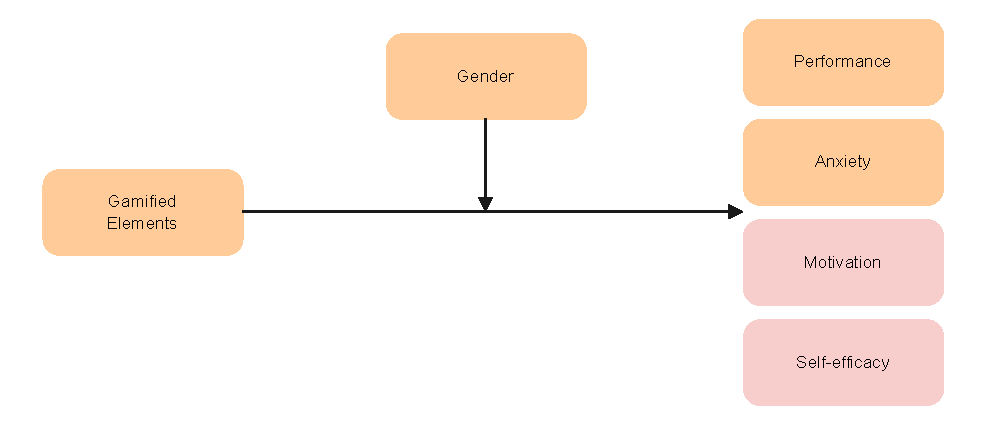
\includegraphics{img/Hypotheses}
    \caption{This diagram illustrates the impact of gamified elements (independent variable) on performance and anxiety (dependent variables), mediated by gender (mediating variable).}
    \label{fig:figureHypotheses}
\end{figure} The hypotheses we want to investigate in this work are:
\begin{itemize}
    \item[H1] Males and females differ in their cognitive and affective states.
    \begin{APAitemize}
        \item[a)] Male performance is better compared to female.
        \item[b)] Male and female students differ regarding their anxiety levels.
    \end{APAitemize}
    \item[H2] Different gamified elements have a varying impact on the cognitive and affective states.
    \begin{APAitemize}
        \item[a)] Gamified elements impact performance differently.
        \item[b)] Different gamified elements impact anxiety levels differently.
    \end{APAitemize}
    \item[H3] Different gamified elements differently impact the cognitive and affective states of males and females.
    \begin{APAitemize}
        \item[a)] The influence of different gamified elements on performance differs between males and females.
        \item[b)] The influence of different gamified elements on anxiety levels differs between males and females.
    \end{APAitemize}
\end{itemize}
\section{Methods}
\subsection{Participants}
117 students were recruited between the 24.06. and the 15.07. from the university campus, with 83 (70.94\%) identifying as male, 34 (29.06\%) as female.
Participants were aged between 18 and 27, with a mean of 21.91 (\textit{SD} = 2.38) years, resulting in an interval of [19.53, 24.29].
The study programs most frequently represented were technical study programs, like Computer Science B.Sc. (n = 34), Software Engineering B.Sc. (n = 11), Aerospace Engineering B.Sc. (n = 8), Mechanical Engineering B.Sc. (n = 7) and Data Science B.Sc. (n = 5).
Participants gave informed consent, each received €15 as monetary compensation for their involvement in the study.

\subsection{Design}
This study employed a 2 $\times$ 8 factorial design, examining the impacts of gamified elements and gender on performance and anxiety within a digital learning environment.
The independent variables were gamified elements and gender.
Gamified elements, included the following eight conditions: No Gamification (None), Points (P), Badges (B), Leaderboards (L), Avatars (A), Narrated Content (N), Points-Badges-Leaderboards-Avatars (PBLA) and Points-Badges-Leaderboards-Avatars-Narrated Content (PBLAN).
The gender variable was measured categorically with participants identifying as male, female, or other.
Each participant experienced three blocks with different gamified elements / conditions, chosen randomly from a pre-generated set to ensure a balanced distribution across conditions.
However, since each participant experienced only three out of the eight possible conditions, and different participants could experience different sets of conditions, this setup integrates elements of both within-subjects and between-subjects designs.
This allowed for the analysis of interaction effects between gamified elements and gender on the dependent variables, which were performance and anxiety.

\subsection{Materials}
\subsubsection{Physical Environment}
The study was conducted in two separate rooms in the cellar of a university building, one equipped with five and one with seven iMacs.
As \textcite{christyLeaderboardsVirtualClassroom2014} suggested that the environment can influence the results, both rooms were equipped with the same furniture and lighting and were furnished like a typical software laboratory.

\subsubsection{Virtual Environment}
The software used in this study was built by the author using SvelteKit in frontend and KTor in backend. Its UI was designed after the study by \textcite{albuquerqueDoesGenderStereotype2017}.
On the iMacs the study was displayed full-screen mode using the Safari web browser to ensure no further distractions. The study consisted of 7 screens.
A consent screen gave an overview and explained the data collection to the user. The consent screen had to be accepted in order to proceed.
The demographic data screen in Figure \ref{fig:figureDetails} collected gender, age and study program. Participants also had to enter a deletion code in order to request their data's deletion after the collection.
\begin{figure}[H]
  \centering
  \includegraphics[width=0.7\textwidth]{img/details.png}
  \caption{The personal details collection form}
  \label{fig:figureDetails}
\end{figure}
The next screen was the gamified learning environment, where the participants had to solve questions while being exposed to the gamified elements.
The matrices were taken from \textcite{albuquerqueDoesGenderStereotype2017}, for example Figure \ref{fig:figureMatrices} (left), to generate 60 questions out of the 20, the 40 questions for iteration two and three were slightly altered versions of the original 20 made by this author.
Those alterations included changing the position or rotation of the elements in the matrix and the five possible answers, for example Figure \ref{fig:figureMatrices} (right).
\begin{figure}[H]
  \centering
  \begin{subfigure}[t]{0.45\textwidth}
    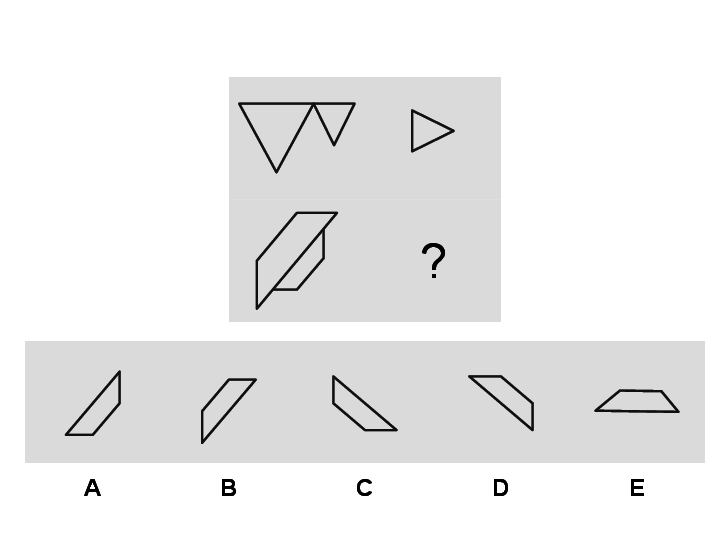
\includegraphics[width=\textwidth]{img/q-17.png}
  \end{subfigure}
  \hspace{5mm}
  \begin{subfigure}[t]{0.45\textwidth}
    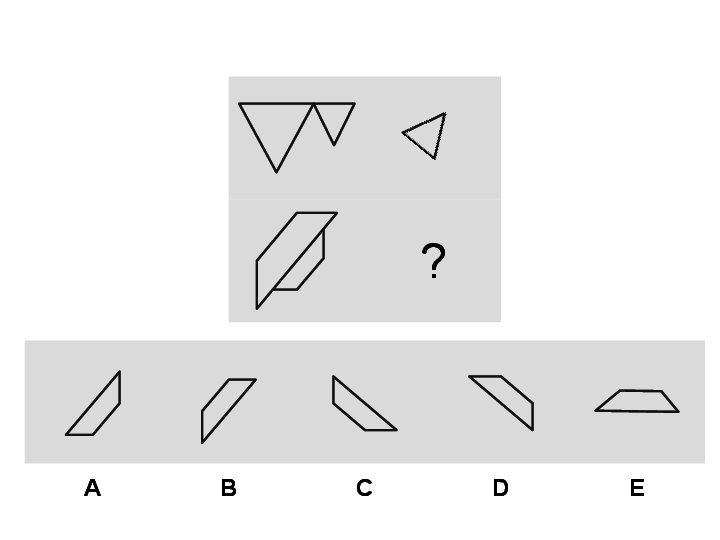
\includegraphics[width=\textwidth]{img/q-57.png}
  \end{subfigure}
  \caption{Left: A standard progressive matrix from \textcite{albuquerqueDoesGenderStereotype2017} given to the participants. Right: A slightly altered version of the same matrix}
  \label{fig:figureMatrices}
\end{figure}
The gamified learning environment \ref{fig:figureScreen} consisted of different UI elements representing the gamified elements.
\begin{APAitemize}
  \item \textbf{Leaderboards}: A list of participants and scores, including the current participant. The list items consisted of rank, name in the format "Player " + random number and score, the players item was highlighted. The other players shown were not real, their scores were randomly generated so that the player started on the sixth place and the first place was always possible.
  \item \textbf{Badges}: An array of four badges that were awarded for 1, 5, 10 and 18 correctly answered questions.
  \item \textbf{Avatars}: A small avatar that was shown in the top right corner of the screen and on the leaderboard. To increase identification with the avatar further, the participants were asked to choose one of 15 different avatars before the iteration.
  \item \textbf{Narrated content}: Narrated content was shown in the bottom right corner of the screen. It was presented as a chat bubble with an avatar next to it, appearing like it spoke, in case avatars were enabled. It showed a random praise or encouragement sentence every three questions.
  \item \textbf{Points}: A counter next to the question frame showed the current points. One point was awarded for each correctly answered question.
\end{APAitemize}
\begin{figure}[H]
  \centering
  \begin{subfigure}[t]{0.4\textwidth}
    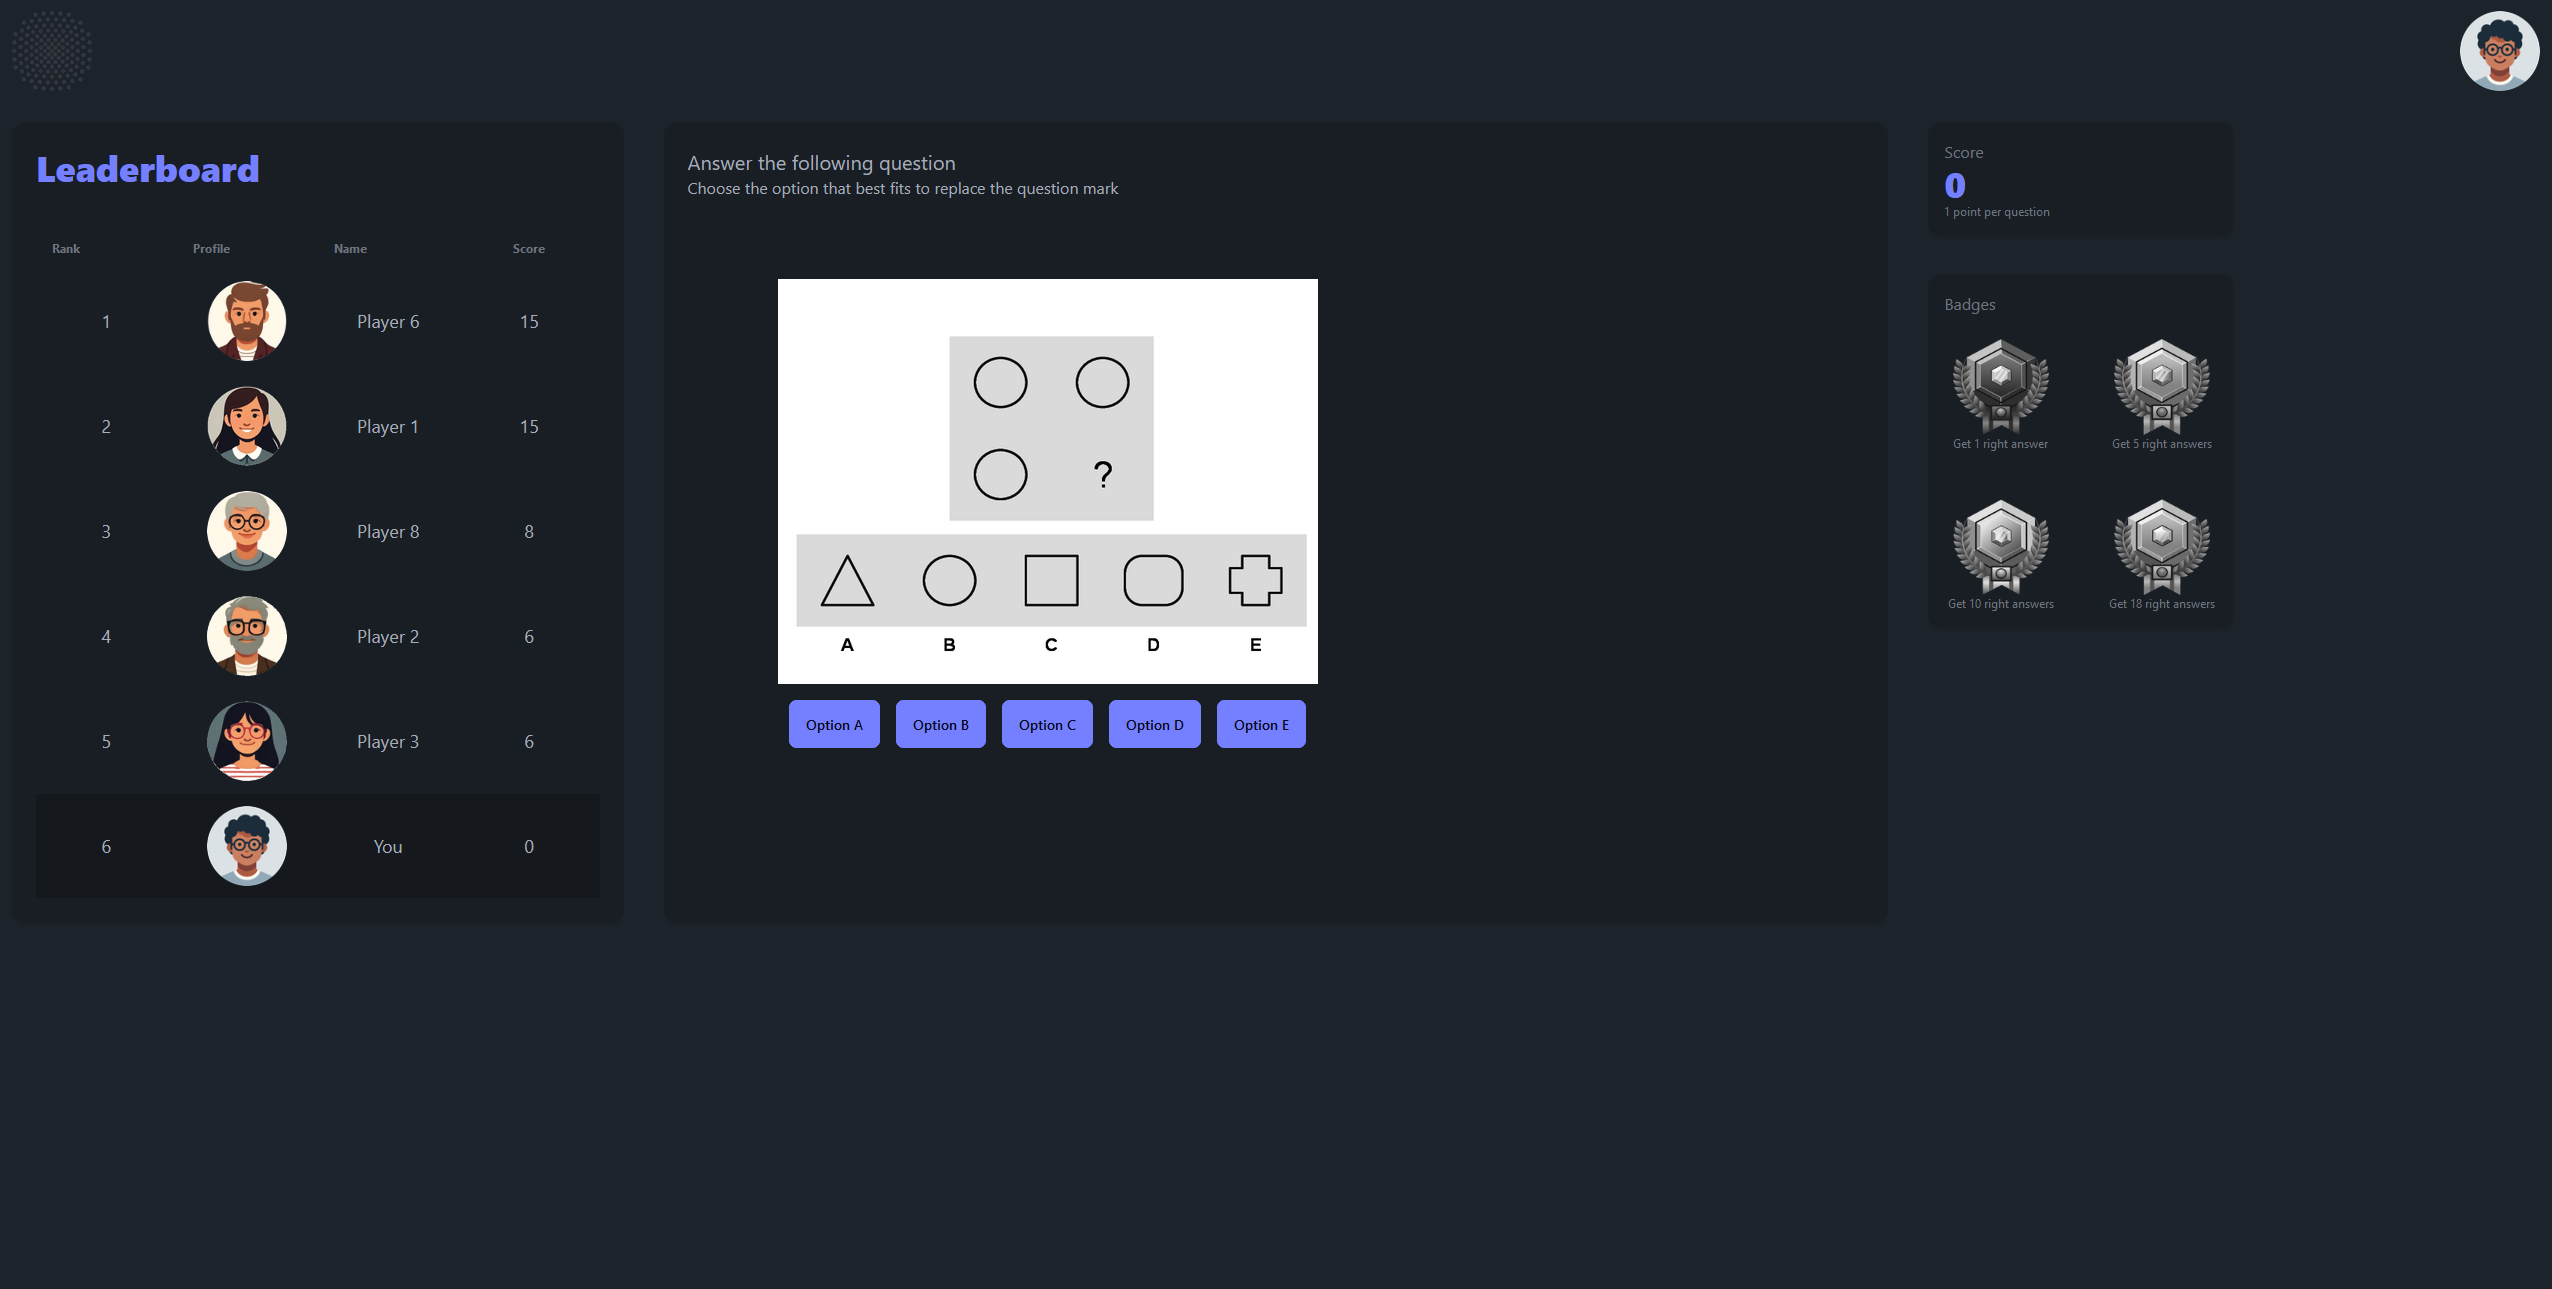
\includegraphics[width=\textwidth]{img/question_screen.png}
    \label{fig:figureScreenEnabled}
  \end{subfigure}
  \hspace{5mm}
  \begin{subfigure}[t]{0.4\textwidth}
    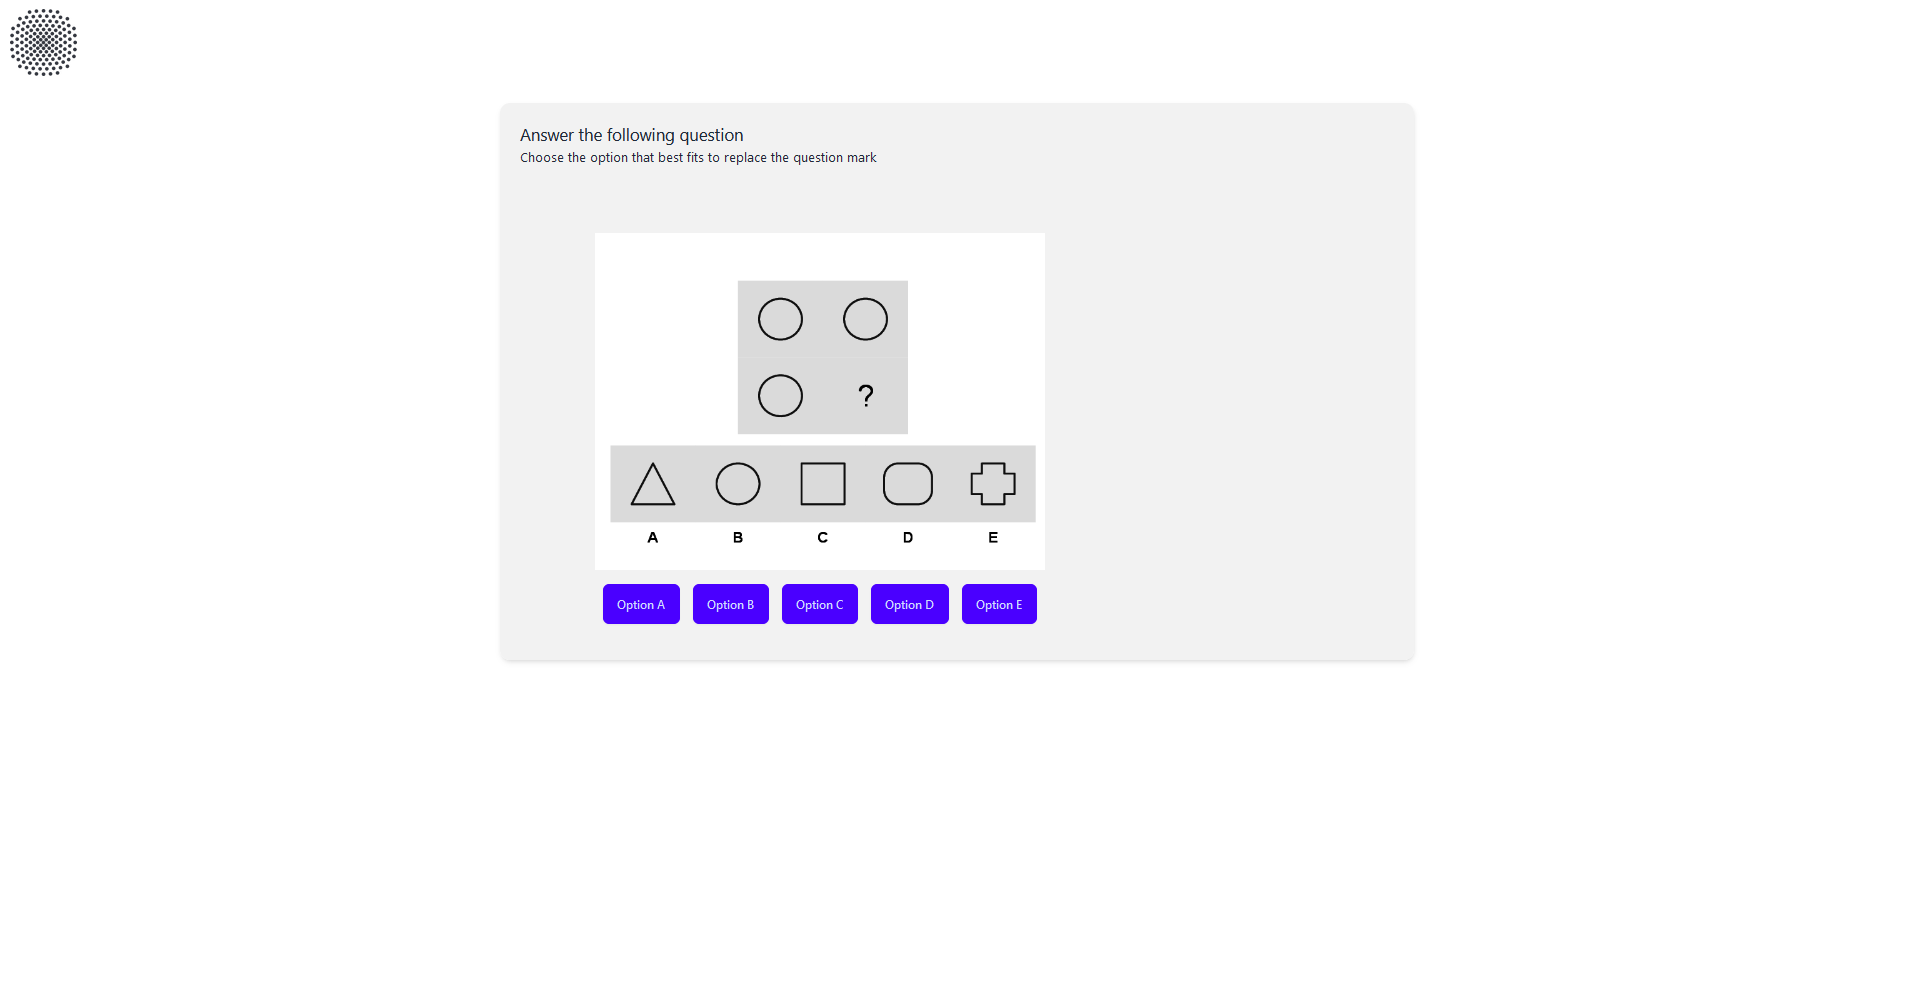
\includegraphics[width=\textwidth]{img/question_screen_no_elements.png}
    \label{fig:figureScreenDisabled}
  \end{subfigure}
  \caption{Comparison of the Digital Learning Environment with gamified elements enabled (left) and without gamified elements enabled (right). Narrated content in only shown between questions so it is not possible to show it in the same screenshot.}
  \label{fig:figureScreen}
\end{figure}

After the gamified learning environment, the participants were shown a questionnaire for anxiety, motivation and self-efficacy.
The three questionnaires were a six-question shortened form of the State-Trait Anxiety Inventory (STAI, \textcite{marteauDevelopmentSixitemShortform1992}), the eight-question General Self-Efficacy Scale (GSE \textcite{guayAssessmentSituationalIntrinsic2000}) and the 16-question Situational Intrinsic Motivation Scale (SIMS, \textcite{chenValidationNewGeneral2001}).
\begin{figure}[H]
  \centering
  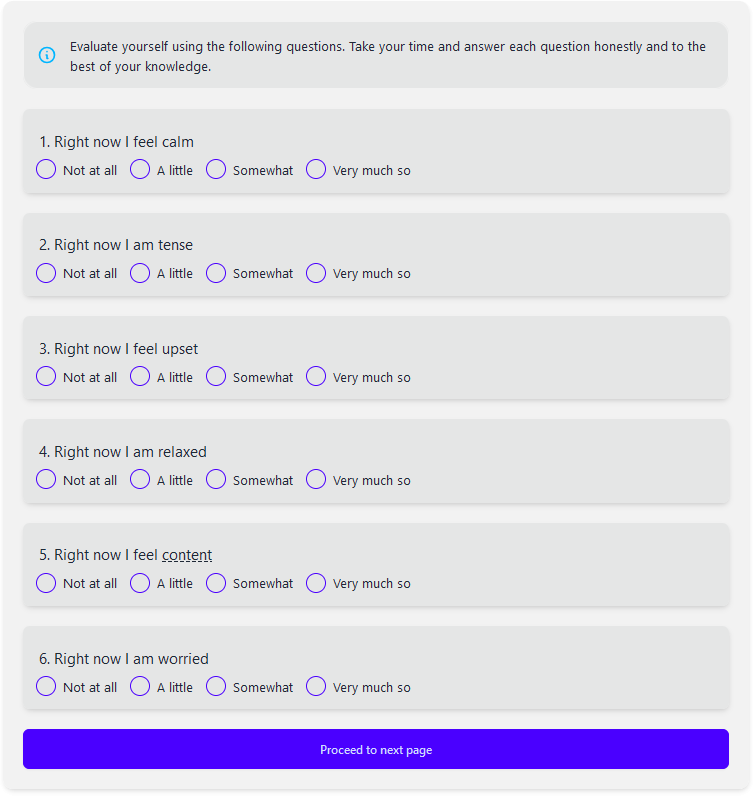
\includegraphics[width=0.4\textwidth]{img/Stai.png}
  \caption{The anxiety questionnaire}
  \label{fig:figureAnxiety}
\end{figure}
To submit data to the backend there was a data submission screen that guided the participants to the next iteration or in case of the third iteration to the end of the study.

\subsection{Procedure}

Participants have been enlisted at the university campus and invited to engage in a study concerning gamification, with an incentive of 15€ offered upfront for their involvement.
Following a brief overview of the study's framework, they have been directed to select both a room and a computer.
The initial screens presented were those seeking consent and outlining the study details and the demographic data collection screen. Subsequently, participants have inputted their demographic data, leading into the three gamified blocks.\\
Each block has initiated with the gamified learning environment, followed by three questionnaires, and concluded with a data submission interface.
After answering one question the next question has a one-second delay which increases to four seconds if narrated content is shown.
The sequence and consistency of the testing procedure, including the series of questions asked in the gamified digital learning environment have always been maintained to ensure the reliability of measurements and comparability of results across the various stages of the experiment.
Participants have been advised to proceed at their own pace and refrain from communicating with fellow participants throughout the duration of the study.
Upon completion of the third iteration, they have been acknowledged for their contribution and compensated with the 15€.
\begin{figure}[H]
  \centering
  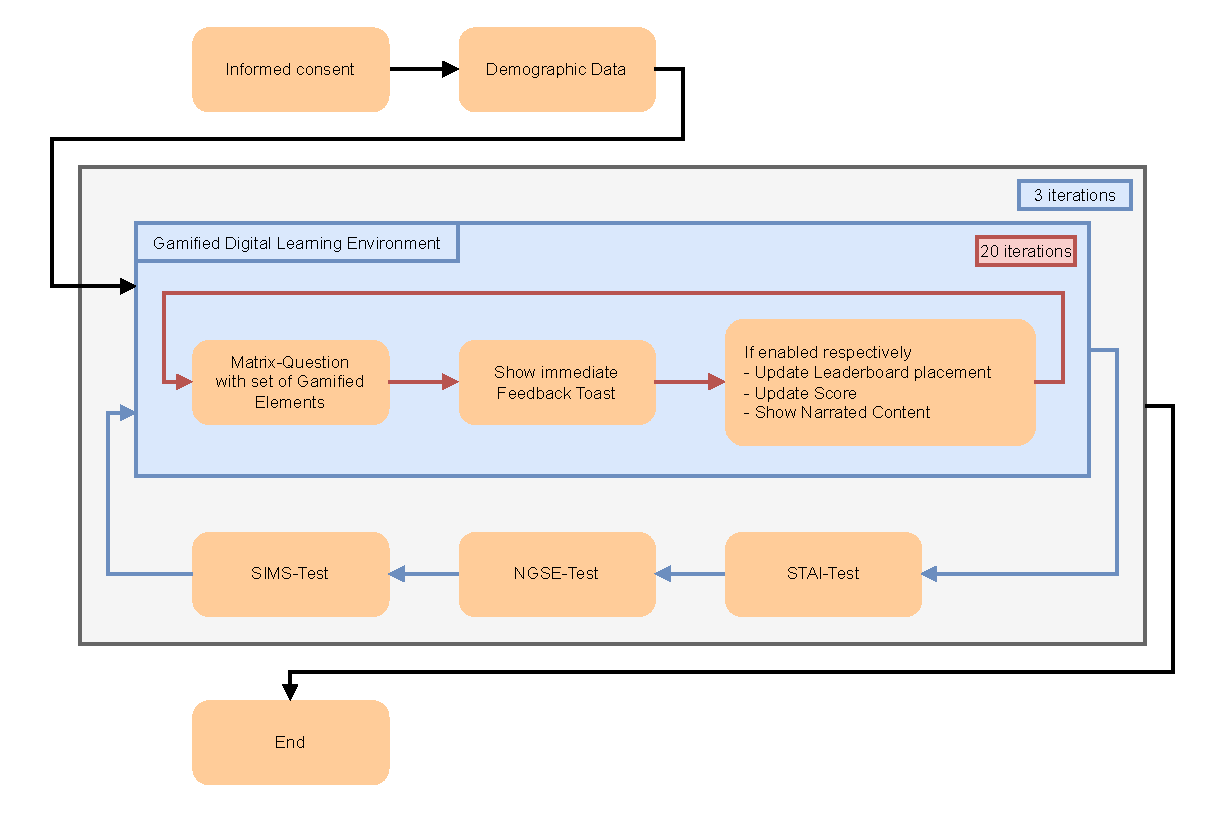
\includegraphics[width=\textwidth]{img/Procedure_alt.pdf}
  \caption{The procedure of the study}
  \label{fig:figureProcedure}
\end{figure}

\subsection{Scoring}

The data was cleaned and processed before analysis to ensure accuracy and reliability. The scores for the different conditions were calculated as follows:

\begin{APAitemize}
\item \textbf{Performance:} The performance was calculated as the ratio of correctly answered questions to the total number of questions.
\item \textbf{State-Trait Anxiety Inventory (STAI):} The STAI scores were calculated using the six-item short-form version of the state scale, as developed by \textcite{marteauDevelopmentSixitemShortform1992}. Participants rated their responses on a scale from "Not at all" to "Very much so," corresponding to numerical values from zero to five. The original test contains both anxiety-present and anxiety-absent items, with appropriate weights applied as per the guidelines by \textcite{marteauDevelopmentSixitemShortform1992}. Negative weights were used for items indicating anxiety (e.g., "Right now I am worried").
\end{APAitemize}
% !TeX spellcheck = en_US

\section{Results}
\label{chap:evaluation}
\subsection{Data Exclusion}
Participants who identified their gender as "other" were excluded from the analysis because the present research available and used for this thesis primarily focuses on comparisons between male and female participants.
This criterion led to the exclusion of two participants. Additionally, participants who achieved less than 25\% correct answers in the gamified learning environment were excluded.
This threshold was set because there were five possible answers for each question, and random clicking would statistically result in a 20\% correct response rate.
Therefore, a performance below 25\% suggests either random guessing or a fundamental misunderstanding of the task.
Furthermore, any incomplete data sets were excluded to ensure the integrity and consistency of the analysis, resulting in the exclusion of one additional participant.
Initially, there were 120 data sets, and after applying the exclusion criteria, 117 data sets remained.

\subsection{Outline of Statistical Analysis}
Having preprocessed and cleaned the data, we proceeded with our statistical analysis using linear mixed models (LMMs).
These models were chosen for their ability to handle the complexities of repeated measures from the same subjects under varying conditions.
By incorporating both fixed effects (gender and gamified elements) and random effects (individual differences), LMMs provided a robust framework for our analysis.

We utilized the Nelder-Mead optimization method to estimate the parameters of our models.
This method is ideal for our needs as it efficiently handles models with multiple interacting effects without requiring derivative calculations, making it suitable for our complex dataset.

For the estimation of variance components within our models, we employed Restricted Maximum Likelihood (REML).
REML is preferred in mixed model contexts because it adjusts the estimates for the fixed effects, providing unbiased variance estimates despite the presence of random effects.

Finally, to ensure accurate inference regarding the fixed effects, we applied the Satterthwaite approximation for estimating degrees of freedom.
This method helps in achieving more reliable p-values by adjusting the degrees of freedom for the complexity of the model, crucial in cases with multiple levels of interactions and a limited sample size.

This combination of methods and their implementation through LMMs allowed us to systematically analyse the effects of gender and gamified elements on performance and anxiety, controlling for individual variability and the specifics of the experimental design.

\subsection{Report of findings}

\subsubsection{Performance}
Women exhibited lower performance levels when leaderboards were the gamified element used (\textit{M}= .700, \textit{SE} = .056) compared to men (\textit{M} = .835, \textit{SE} = .024) and to the overall average performance in gamified settings for women (\textit{M} = .846, \textit{SE} = 0.030).
Notable is also the variability suggested by the large standard error for women in this leaderboard condition.
Despite some descriptive effects, our analysis revealed no significant main effects or interactions for all hypotheses regarding performance, as documented in \autoref{tab:lmm_performance}.

\begin{figure}[h]
    \centering
    \begin{subfigure}[b]{0.45\textwidth}
        \includegraphics[width=\textwidth]{img/plots/grey/plot_performance.png}
        \label{fig:plot_performance}
    \end{subfigure}
    \hfill
    \begin{subfigure}[b]{0.45\textwidth}
        \includegraphics[width=\textwidth]{img/plots/grey/plot_performance_gender.png}
        \label{fig:plot_performance_gender}
    \end{subfigure}
    \caption{On the left: Overall performance across different gamification elements as percentage. On the right: Performance by gender grouped by gamification element as percentage.}
    \label{fig:performance_comparison}
\end{figure}

\begin{table}[h]
    \centering
    \caption{Results of the linear mixed model analysis for percentage correct effects.}
    \label{tab:lmm_performance}
    \begin{tabular}{lcccc}
        \hline
        Variable & \textit{beta} & \textit{p} & \textit{t} & \textit{df} \\
        \hline
        m & 0.07 & .994 & 0.27 & 277.62 \\
        P & -0.33 & .493 & -1.35 & 211.82 \\
        B & 0.06 & .994 & 0.21 & 214.27 \\
        L & -0.48 & .384 & -1.67 & 213.69 \\
        A & 0.13 & .994 & 0.49 & 208.19 \\
        N & 0.44 & .384 & 1.70 & 207.03 \\
        PBLA & 0.01 & .994 & 0.06 & 208.37 \\
        PBLAN & 0.06 & .994 & 0.22 & 210.22 \\
        m $\times$ P & 0.42 & .493 & 1.33 & 214.33 \\
        m $\times$ B & -0.22 & .994 & -0.64 & 213.78 \\
        m $\times$ L & 0.61 & .384 & 1.79 & 214.82 \\
        m $\times$ A & 0.01 & .994 & 0.03 & 209.52 \\
        m $\times$ N & -0.00 & .994 & -0.01 & 210.19 \\
        m $\times$ PBLA & 0.37 & .548 & 1.18 & 211.59 \\
        m $\times$ PBLAN & 0.01 & .994 & 0.02 & 210.43 \\
        \hline
    \end{tabular}
    \tablenote{Abbreviations: m = Male, P = Points, B = Badges, L = Level, A = Avatars, N = Narrative Content, PBLA = Combination of Points, Badges, Level, and Avatars, PBLAN = Combination of all elements. Male is compared to female performance, gamified elements are compared to the non-gamified environment. The interactions are compared to female in the non-gamified environment.}
\end{table}




\subsubsection{Anxiety}
Some descriptive trends emerged from our analysis, as illustrated in \autoref{fig:anxiety_comparison}.
Women experienced higher anxiety levels than men in the non-gamified environment (\textit{M} = .571, \textit{SE} = .092 for women compared to \textit{M} = .296, \textit{SE} = .099 for men) and when leaderboards were used (\textit{M} = .683, \textit{SE} = .205 for women compared to \textit{M} = .566, \textit{SE} = .119 for men).
In contrast, the use of avatars was associated with lower anxiety levels for women (\textit{M} = .187, \textit{SE} = .095) than for men (\textit{M} = .476, \textit{SE} = .102).

Despite these trends, our analysis revealed no significant main effects or interactions for any of the hypotheses regarding anxiety levels, as detailed in \autoref{tab:lmm_stai}.
This leads us to conclude that the hypotheses regarding anxiety must be rejected.


\begin{figure}[h]
    \centering
    \begin{subfigure}[b]{0.45\textwidth}
        \includegraphics[width=\textwidth]{img/plots/grey/plot_anxiety.png}
    \end{subfigure}
    \hfill
    \begin{subfigure}[b]{0.45\textwidth}
        \includegraphics[width=\textwidth]{img/plots/grey/plot_anxiety_gender.png}
    \end{subfigure}
    \caption{On the left: Anxiety levels across different gamification elements. On the right: Differences in anxiety levels by gender grouped by gamified element.}
    \label{fig:anxiety_comparison}
\end{figure}

\begin{table}[h]
    \centering
    \caption{Results of the linear mixed model analysis for STAI effects.}
    \label{tab:lmm_stai}
    \begin{tabular}{lccccc}
        \hline
        Variable & \textit{beta} & \textit{p} & \textit{t} & \textit{df} \\
        \hline
        m & -0.25 & .623 & -0.83 & 288.25 \\
        P & -0.28 & .564 & -1.00 & 216.76 \\
        B & 0.23 & .623 & 0.73 & 221.07 \\
        L & -0.04 & .913 & -0.11 & 220.38 \\
        A & -0.62 & .228 & -2.11 & 213.37 \\
        N & -0.53 & .241 & -1.81 & 211.70 \\
        PBLA & -0.03 & .913 & -0.11 & 213.53 \\
        PBLAN & -0.60 & .228 & -2.04 & 215.77 \\
        m $\times$ P & 0.42 & .481 & 1.18 & 220.20 \\
        m $\times$ B & -0.18 & .787 & -0.47 & 220.26 \\
        m $\times$ L & 0.28 & .623 & 0.74 & 221.54 \\
        m $\times$ A & 0.64 & .241 & 1.79 & 214.84 \\
        m $\times$ N & 0.50 & .437 & 1.40 & 215.47 \\
        m $\times$ PBLA & 0.10 & .882 & 0.29 & 217.43 \\
        m $\times$ PBLAN & 0.45 & .481 & 1.25 & 215.91 \\
        \hline
    \end{tabular}
    \tablenote{Abbreviations: m = Male, P = Points, B = Badges, L = Leaderboards, A = Avatars, N = Narrative Content, PBLA = Combination of Points, Badges, Leaderboards, and Avatars, PBLAN = Combination of all elements. Male is compared to female anxiety, gamified elements are compared to the non-gamified environment. The interactions are compared to female in the non-gamified environment.}
\end{table}
\section{Discussion}
\subsection{Summary of Research focus}
This thesis explored the effects of gamification elements on performance and anxiety in digital learning environments, with a focus on gender differences.
Using a randomized controlled design, the study assessed various gamification components like points, badges, leaderboards, and avatars, analysing responses from male and female participants.
The main goal was to identify how different genders react to these gamification strategies regarding their cognitive and affective states.

Although the study did not find statistically significant effects, the data trends were in line with existing research, indicating consistent patterns in how participants reacted to the gamification elements.
This suggests that while the effects were not strong enough to be statistically significant, the observed behaviours reflected known theories and previous studies.
These results highlight the challenges of isolating the impacts of gamification and gender in educational contexts, pointing to the potential need for further research with larger sample sizes or different approaches.
\subsection{Interpretation of Results}
The absence of statistically significant findings in this study does not negate the observation of certain trends that suggest a subtle influence of gamification on learning outcomes.
These observed trends align with previous research that also noted similar patterns without definitive effects \parencite{dehghanzadehUsingGamificationSupport2024,hamariDoesGamificationWork2014}.
This consistency suggests that while the direct impact of gamified elements may not be significant in our study, there is a consistent directional influence on learners' cognitive and affective states.
This highlights the nuanced nature of gamification effects, suggesting that they may manifest under specific conditions or within certain contexts, as \textcite{dehghanzadehUsingGamificationSupport2024,koivistoRiseMotivationalInformation2019}.

\subsection{Implications for Theory and Practice}
Theoretically, the observed trends, hint at potential variations in how gamification impacts different learners, suggesting a need for broader conceptual models.
This could inspire further research into personalized learning environments.
Practically, these preliminary findings encourage a cautious approach to integrating gamification in educational settings.
Designers might consider more flexible gamification systems that can be adjusted based on learner feedback, potentially enhancing user engagement without a one-size-fits-all strategy.


\subsection{Limitations}
This study has several key limitations that must be acknowledged. Firstly, the reliance on self-reported data from students may lead to potential biases and inaccuracies in the findings. Previous research suggests that objective measures, such as sensor-based tracking, could provide more reliable data \parencite{woolfAffectiveTutorsAutomatic2010}.
Another significant limitation arises from the demographic and location constraints of our sample. The majority of participants were recruited from the computer science building on a technical campus, which may not provide a diverse representation of the general student population.
Additionally, the customization options for avatars were limited, lacking diverse representations such as Hijabs or beards, as noted by participants. This limitation may affect the engagement and identification of users with the avatars, potentially skewing the results regarding the impact of gamification on different genders.
The narrated content of the gamified elements could also be not engaging enough, being confined to a small portion of the screen without integrating characteristics, abilities, or dialogues that could enhance user interaction. This might have contributed to some participants opting to disable gamified elements, thus not experiencing the intended gamified environment fully.
Furthermore, the design of the study involved three iterations per participant, which might have led to habituation effects. These effects could influence the outcomes in terms of learning environment adaptability, anxiety, motivation, and self-efficacy, thus potentially diminishing the study's ability to measure these constructs accurately over time.
Finally, the lack of sufficient individualized feedback post-study was highlighted as a concern. Future iterations of this study should consider incorporating mechanisms for more personalized and actionable feedback to enhance the learning and adaptation process for participants.
Despite these limitations, the findings provide valuable insights into the intersection of gamification and gender, suggesting avenues for future research and practical applications in educational environments.

\section{Future Research}
As highlighted in the introduction, the exploration of individual characteristics in the selection of gamified elements within learning environments requires further investigation. This thesis has laid foundational insights into how gender influences engagement with gamified systems. However, other dimensions such as age, culture, and notably, the educational level (ranging from school-level to higher education and adult learning) merit in-depth exploration to comprehensively understand the dynamics at play.

Moreover, while the study's learning environment provided a basic platform, it does not directly represent the probable application of gamified elements. As noted earlier, gamified elements are prevalently integrated into Intelligent Tutoring Systems. Therefore, conducting studies that focus on gamified ITS can yield more pertinent insights into their efficacy and application.
As the modelling of such systems, even without gamification, is quite extensive and customizable per learner itself, for it to work properly, it should be tested in an ITS.

Additionally, the temporal scope of this study was limited, addressing only short-term interactions. Prior research has established the significance of longitudinal studies in this domain \parencite{oliveiraTailoredGamificationEducation2023,dehghanzadehUsingGamificationSupport2024}. Extending research timelines to span multiple semesters would provide a more robust understanding of the long-term impacts of gamification on learning outcomes and student engagement. Such extended studies are quite challenging in every research area, but crucial for observing changes in learner stategies and behaviour and the sustainability of gamification benefits over time.

In conclusion, advancing research in these areas will not only enrich our understanding of how different groups respond to gamified learning but also enhance the design and implementation of educational technologies that are inclusive and effective across diverse learning environments.

\subsection*{Conclusion}
This study's exploration into the effects of gamification elements on performance and anxiety with a focus on gender differences has provided initial insights that, while not statistically significant, point to subtle yet potentially important trends.
The observed data suggest that certain gamified elements could have differential impacts on cognitive and affective outcomes across genders.
Although these effects were not strong enough to achieve statistical significance in this study, the descriptive findings hint at underlying patterns that merit further investigation.

The consistency of these patterns with prior research indicates that with improved research designs that address the limitations of this study, significant findings could be obtained.
These findings could be very important for advancing the understanding of how gamification can be optimized to enhance performance and anxiety effectively.
Future research should consider these aspects to uncover more robust evidence that can contribute to the ongoing discourse in educational technology.


\subsection*{Acknowledgements}
We acknowledge the support of the German Research Foundation (DFG; DFG reference number UP 31/1) for funding the Stuttgart Research Focus Interchange Forum for Reflecting on Intelligent Systems (IRIS).
This research was further supported by the Ministry of Science, Research, and the Arts (MWK) Baden-Württemberg, Germany, within the Artificial Intelligence Software Academy (AISA; reference number Az. 7542.2-9-47.10/36/2).

\printbibliography

\end{document}

%% 
%% Copyright (C) 2021 by Daniel A. Weiss <daniel.weiss.led at gmail.com>
%% 
%% This work may be distributed and/or modified under the
%% conditions of the LaTeX Project Public License (LPPL), either
%% version 1.3c of this license or (at your option) any later
%% version.  The latest version of this license is in the file:
%% 
%% http://www.latex-project.org/lppl.txt
%% 
%% Users may freely modify these files without permission, as long as the
%% copyright line and this statement are maintained intact.
%% 
%% This work is not endorsed by, affiliated with, or probably even known
%% by, the American Psychological Association.
%% 
%% 
%% This work is "maintained" (as per LPPL maintenance status) by
%% Daniel A. Weiss.
%% 
%% This work consists of the file  apa7.dtx
%% and the derived files           apa7.ins,
%%                                 apa7.cls,
%%                                 apa7.pdf,
%%                                 README,
%%                                 APA7american.txt,
%%                                 APA7british.txt,
%%                                 APA7dutch.txt,
%%                                 APA7english.txt,
%%                                 APA7french.txt,
%%                                 APA7german.txt,
%%                                 APA7ngerman.txt,
%%                                 APA7greek.txt,
%%                                 APA7czech.txt,
%%                                 APA7turkish.txt,
%%                                 APA7endfloat.cfg,
%%                                 Figure1.pdf,
%%                                 shortsample.tex,
%%                                 longsample.tex, and
%%                                 bibliography.bib.
%% 
%%
%% End of file `./samples/longsample.tex'.